%definira klasu dokumenta 
\documentclass[12pt]{report} 

%prostor izmedu naredbi \documentclass i \begin{document} se zove uvod. U njemu se nalaze naredbe koje se odnose na cijeli dokument

%osnovni LaTex ne može riješiti sve probleme, pa se koriste različiti paketi koji olakšavaju izradu željenog dokumenta
\usepackage[croatian]{babel} 
\usepackage{amssymb}
\usepackage{amsmath}
\usepackage{txfonts}
\usepackage{mathdots}
\usepackage{titlesec}
\usepackage{array}
\usepackage{lastpage}
\usepackage{etoolbox}
\usepackage{longtable, tabu}
\usepackage{color, colortbl}
\usepackage{adjustbox}
\usepackage{geometry}
\usepackage[classicReIm]{kpfonts}
\usepackage{hyperref}
\usepackage{fancyhdr}

\usepackage{float}
\usepackage{setspace}
\restylefloat{table}


\patchcmd{\chapter}{\thispagestyle{plain}}{\thispagestyle{fancy}}{}{} %redefiniranje stila stranice u paketu fancyhdr

%oblik naslova poglavlja
\titleformat{\chapter}{\normalfont\huge\bfseries}{\thechapter.}{20pt}{\Huge}
\titlespacing{\chapter}{0pt}{0pt}{40pt}


\linespread{1.3} %razmak između redaka

\geometry{a4paper, left=1in, top=1in,}  %oblik stranice

\hypersetup{ colorlinks, citecolor=black, filecolor=black, linkcolor=black,	urlcolor=black }   %izgled poveznice


%prored smanjen između redaka u nabrajanjima i popisima
\newenvironment{packed_enum}{
	\begin{enumerate}
		\setlength{\itemsep}{0pt}
		\setlength{\parskip}{0pt}
		\setlength{\parsep}{0pt}
	}{\end{enumerate}}

\newenvironment{packed_item}{
	\begin{itemize}
		\setlength{\itemsep}{0pt}
		\setlength{\parskip}{0pt}
		\setlength{\parsep}{0pt}
	}{\end{itemize}}


%boja za privatni i udaljeni kljuc u tablicama
\definecolor{LightBlue}{rgb}{0.9,0.9,1}
\definecolor{LightGreen}{rgb}{0.9,1,0.9}


%podesavanje zaglavlja i podnožja

\pagestyle{fancy}
\lhead{Programsko inženjerstvo}
\rhead{$<$Projektni zadatak$>$}
\lfoot{$<$Naziv grupe$>$}
\cfoot{stranica \thepage/\pageref{LastPage}}
\rfoot{\today}
\renewcommand{\headrulewidth}{0.2pt}
\renewcommand{\footrulewidth}{0.2pt}


\begin{document} 
	
	
	
	\begin{titlepage}
		\begin{center}
			\vspace*{\stretch{1.0}} %u kombinaciji s ostalim \vspace naredbama definira razmak između redaka teksta
			\LARGE Programsko inženjerstvo\\
			\large Ak. god. 2020./2021.\\
			
			\vspace*{\stretch{3.0}}
			
			\huge Kamp „Mlade nade“\\
			\Large Dokumentacija, Rev. \textit{1}\\
			
			\vspace*{\stretch{12.0}}
			\normalsize
			Grupa: \textit{
				FantasticFourPlusThree}\\
			Voditelj: \textit{Dario Strunjak}\\
			
			
			\vspace*{\stretch{1.0}}
			Datum predaje: \textit{$<$dan$>$. $<$mjesec$>$. $<$godina$>$.}\\
	
			\vspace*{\stretch{4.0}}
			
			Nastavnik: \textit{Eugen Vušak, mag. ing. comp}\\
		
		\end{center} 

	
	\end{titlepage}

	
	\tableofcontents

	\chapter{Dnevnik promjena dokumentacije}
		
		\textbf{\textit{Kontinuirano osvježavanje}}\\
				
		
		\begin{longtabu} to \textwidth {|X[2, l]|X[13, l]|X[3, l]|X[3, l]|}
			\hline \multicolumn{1}{|l|}{\textbf{Rev.}}	& \multicolumn{1}{l|}{\textbf{Opis promjene/dodatka}} & \multicolumn{1}{|l|}{\textbf{Autori}} & \multicolumn{1}{l|}{\textbf{Datum}} \\[3pt] \hline
			\endfirsthead
			
			\hline \multicolumn{1}{|l|}{\textbf{Rev.}}	& \multicolumn{1}{l|}{\textbf{Opis promjene/dodatka}} & \multicolumn{1}{|l|}{\textbf{Autori}} & \multicolumn{1}{l|}{\textbf{Datum}} \\[3pt] \hline
			\endhead
			
			\hline 
			\endlastfoot
			
			0.1 & Napravljen predložak.	& Došen & 12.10.2020. 		\\[3pt] \hline 
			0.2	& Dodani opis projektnog zadatka i funkcionalni zahtjevi. & Došen & 13.10.2020. 	\\[3pt] \hline 
			0.2.1 & Ispravak opisa zadatka, funkcionalnih zahtjeva i predloška. & Strunjak & 13.10.2020. 	\\[3pt] \hline 
			0.3 & Dodan popis obrazaca uporabe & Strunjak & 20.10.2020. 	\\[3pt] \hline 
			0.3.1 & Popunjeni obrasci uporabe UC31-UC40 & Strunjak & 20.10.2020. 	\\[3pt] \hline
			0.3.1 & Popunjeni obrasci uporabe UC7-UC12 & Deković & 21.10.2020. 	\\[3pt] \hline
			0.3.1 & Popunjeni obrasci uporabe UC19-UC24 & Došen & 21.10.2020. 	\\[3pt] \hline
			0.3.1 & Popunjeni obrasci uporabe UC25-UC30 & Vicković & 21.10.2020.  \\[3pt]  \hline
			0.3.1 & Popunjeni obrasci uporabe UC1-UC6 & Dolić & 22.10.2020. 	\\[3pt] \hline
			0.3.2 & Napravljen i dodan UC dijagram za organizatora & Deković & 22.10.2020. 	\\[3pt] \hline
		\end{longtabu}
	
	
	 
	\chapter{Opis projektnog zadatka}
		
		\textbf{\textit{dio 1. revizije}}\\
		
		\textit{Cilj ovog projekta je razviti online platformu za upravljanje i organizaciju kampa računarstva „Mlade nade“. Platforma će davati uvid u raspored, aktivnosti, te podatke o grupama i njenim članovima. Potencijalna korist ovog projekta jest jednostavnija organizacija kampa, te digitalizacija prijava na kamp, iz čega slijedi potencijalno veći broj prijavljenjih.}
		
		\textit{Sustav omogućava funkcionalnosti za 3 dionika: organizator, sudionik i animator. Neprijavljeni korisnici mogu vidjeti osnovne informacije o kampu, poput vremena održavanja, trajanja i aktivnosti. Za vrijeme prijava na kamp, na platformi će biti dostupne prijave na kamp za sudionike i/ili animatore. Animatori i sudionici prilikom prijave na kamp unose sljedeće podatke:}
		\begin{packed_item}
			\item \textit{ime i prezime}
			\item \textit{email adresa}
			\item \textit{broj telefona}
			\item \textit{datum i godina rođenja}
			\item \textit{motivacijsko pismo}
			\item \textit{broj odgovorne osobe (samo za sudionike mlađe od 18 godina)}
		\end{packed_item}
	
		\textit{Ako je nečija prijava prihvaćena, tu osobu se o tome obaviještava emailom te joj se šalju podatci potrebni za registraciju na platformu. Ako je nečija prijava odbijena, osoba se o tome također obavještava emailom. Korisnici zatim prilikom registracije za dobiveno korisničko ime (putem maila) upisuju lozinku.}
		
		\textit{Sudionici i animatori nakon prijave u sustav (prije početka kampa) vide samo odbrojavanje do početka kampa i imaju mogućnost kontaktiranja organizatora. Nakon početka kampa (za oba tipa korisnika) vodi na stranicu koja pokazuje njihov raspored ili agendu. Sudionici vide popis članova svoje grupe (u kojoj će sudjelovati na svim aktivnostima) i njihove kontakt podatke, kao i animatore s kojima će raditi i njihove kontakt podatke. Animatori vide popis svih grupa, njihovih članova i drugih animatora, kao i nihove kontakt podatke. Dodatno i sudionici i animatori vide popis aktivnosti na kojima su sudjelovali te imaju opciju ocjenjivanja aktivnosti te ostavljanja kratkog opisa njihovog dojma s aktivnošću. Nakon što je kamp završio, sudionici i animatori mogu ocjeniti i ostaviti vlastiti dojam za cjelokupno iskustvo. }
		
		\textit{Organizatori mogu uređivati osnovne informacije s početne stranice. Oni definiraju aktivnosti, te zadaju vrijeme prijava na kamp za sudionike i animatore. Također, vide popis prijava koje mogu prihvatiti ili odbiti. Organizatori određuju broj grupa u koje će, nakon završetka prijava na kamp, sustav slučajnim odabirom razvrstati sudionike, te ih naknadno mogu ručno razmještati. Organizatori mogu puniti raspored s aktivnostima, aktivnostima pridružiti animatore, te imaju popis svih povratnih ocjena po aktivnostima, koje mogu pretraživati po različitim atributima. Osim povratnih ocjena, organizatori mogu vidjeti popis svih aktivnosti, grupa, te registriranih korisnika, koje mogu uređivati. } 
		
		
		\eject
		
		\section{Primjeri u \LaTeX u}
		
		\textit{Ovo potpoglavlje izbrisati.}\\

		U nastavku se nalaze različiti primjeri kako koristiti osnovne funkcionalnosti \LaTeX a koje su potrebne za izradu dokumentacije. Za dodatnu pomoć obratiti se asistentu na projektu ili potražiti upute na sljedećim web sjedištima:
		\begin{itemize}
			\item Upute za izradu diplomskog rada u \LaTeX u - \url{https://www.fer.unizg.hr/_download/repository/LaTeX-upute.pdf}
			\item \LaTeX\ projekt - \url{https://www.latex-project.org/help/}
			\item StackExchange za Tex - \url{https://tex.stackexchange.com/}\\
		
		\end{itemize} 	


		
		\noindent \underbar{podcrtani tekst}, \textbf{podebljani tekst}, 	\textit{nagnuti tekst}\\
		\noindent \normalsize primjer \large primjer \Large primjer \LARGE {primjer} \huge {primjer} \Huge primjer \normalsize
				
		\begin{packed_item}
			
			\item  primjer
			\item  primjer
			\item  primjer
			\item[] \begin{packed_enum}
				\item primjer
				\item[] \begin{packed_enum}
					\item[1.a] primjer
					\item[b] primjer
				\end{packed_enum}
				\item primjer
			\end{packed_enum}
			
		\end{packed_item}
		
		\noindent primjer url-a: \url{https://www.fer.unizg.hr/predmet/proinz/projekt}
		
		\noindent posebni znakovi: \# \$ \% \& \{ \} \_ 
		$|$ $<$ $>$ 
		\^{} 
		\~{} 
		$\backslash$ 
		
		\begin{longtabu} to \textwidth {|X[8, l]|X[8, l]|X[16, l]|} %definicija širine tablice, širine stupaca i poravnanje
			
			%definicija naslova tablice
			\hline \multicolumn{3}{|c|}{\textbf{naslov unutar tablice}}	 \\[3pt] \hline
			\endfirsthead
			
			%definicija naslova tablice prilikom prijeloma
			\hline \multicolumn{3}{|c|}{\textbf{naslov unutar tablice}}	 \\[3pt] \hline
			\endhead
			
			\hline 
			\endlastfoot
			
			\rowcolor{LightGreen}IDKorisnik & INT	&  	Lorem ipsum dolor sit amet, consectetur adipiscing elit, sed do eiusmod  	\\ \hline
			korisnickoIme	& VARCHAR &   	\\ \hline 
			email & VARCHAR &   \\ \hline 
			ime & VARCHAR	&  		\\ \hline 
			\cellcolor{LightBlue} primjer	& VARCHAR &   	\\ \hline 
			
		\end{longtabu}
		

		\begin{table}[H]
			
			\begin{longtabu} to \textwidth {|X[8, l]|X[8, l]|X[16, l]|} 
				
				\hline 
				\endfirsthead
				
				\hline 
				\endhead
				
				\hline 
				\endlastfoot
				
				\rowcolor{LightGreen}IDKorisnik & INT	&  	Lorem ipsum dolor sit amet, consectetur adipiscing elit, sed do eiusmod  	\\ \hline
				korisnickoIme	& VARCHAR &   	\\ \hline 
				email & VARCHAR &   \\ \hline 
				ime & VARCHAR	&  		\\ \hline 
				\cellcolor{LightBlue} primjer	& VARCHAR &   	\\ \hline 
				
				
			\end{longtabu}
	
			\caption{\label{tab:referencatablica} Naslov ispod tablice.}
		\end{table}
		
		
		%unos slike
		\begin{figure}[H]
			\includegraphics[scale=0.4]{slike/aktivnost.PNG} %veličina slike u odnosu na originalnu datoteku i pozicija slike
			\centering
			\caption{Primjer slike s potpisom}
			\label{fig:promjene}
		\end{figure}
		
		\begin{figure}[H]
			\includegraphics[width=.9\linewidth]{slike/aktivnost.PNG} %veličina u odnosu na širinu linije
			\caption{Primjer slike s potpisom 2}
			\label{fig:promjene2} %label mora biti drugaciji za svaku sliku
		\end{figure}
		
		Referenciranje slike \ref{fig:promjene2} u tekstu.
		
		\eject
		
	
	\chapter{Specifikacija programske potpore}
		
	\section{Funkcionalni zahtjevi}
			
			\textbf{\textit{dio 1. revizije}}\\
			
			\textit{Navesti \textbf{dionike} koji imaju \textbf{interes u ovom sustavu} ili  \textbf{su nositelji odgovornosti}. To su prije svega korisnici, ali i administratori sustava, naručitelji, razvojni tim.}\\
				
			\textit{Navesti \textbf{aktore} koji izravno \textbf{koriste} ili \textbf{komuniciraju sa sustavom}. Oni mogu imati inicijatorsku ulogu, tj. započinju određene procese u sustavu ili samo sudioničku ulogu, tj. obavljaju određeni posao. Za svakog aktora navesti funkcionalne zahtjeve koji se na njega odnose.}\\
			
			
			\noindent \textbf{Dionici:}
			
			\begin{packed_enum}
				
				\item Sudionik
				\item Animator				
				\item Organizator
				
			\end{packed_enum}
			
			\noindent \textbf{Aktori i njihovi funkcionalni zahtjevi:}
			
			
			\begin{packed_enum}
				\item  \underbar{Neregistrirani/neprijavljeni korisnik (inicijator) može:}
				
				\begin{packed_enum}
					
					\item pregledati osnovne informacije o kampu
					\item prijaviti se na kamp (u kapacitetu sudionika ili animatora)
					\item  registrirati se u sustav pomoću podataka dobivenih mailom
					\item prijaviti se u sustav s korisničkim imenom i lozinkom
				\end{packed_enum}
			
				\item  \underbar{Korisnik (sudionik, organizator, animator)(inicijator) može:}
				
				\begin{packed_enum}
					
					\item pregledavati i mijenjati svoje korisničke podatke
					\item izbrisati svoj korisnički račun
					
				\end{packed_enum}
					\item  \underbar{Sudionik, animator (inicijator) može:}
				\begin{packed_enum}
					
					\item vidjeti odbrojavanje do početka kampa (prije početka kampa)
					\item kontaktirati organizatora (prije početka kampa)
					\item pregledati svoj raspored aktivnosti i agendu
					\item vidjeti popis aktivnosti na kojima je sudjelovao te ih ocjeniti i ostaviti komentar
					\item uređivati ostavljenu ocjenu i komentar
					\item po završetku kampa ocjeniti i ostaviti komentar za cjelokupno iskustvo
					
				\end{packed_enum}
					\item  \underbar{Sudionik (inicijator) može:}
				\begin{packed_enum}
					
				    \item vidjeti svoju grupu, popis njenih članova, i njihove kontakt podatke, kao i animatora s kojima će raditi/je radio te njihove kontakt podatke
					
				\end{packed_enum}
					\item  \underbar{Animator (inicijator) može:}
				\begin{packed_enum}
					
					\item vidjeti popis svih grupa, njihovih članova i drugih animatora, kao i njihove kontakt podatke
				
				\end{packed_enum}
					\item  \underbar{Baza podataka (sudionik) može:}
				\begin{packed_enum}
					
					\item pohraniti sve podatke o korisnicima, aktivnostima, grupama i ocjenjivanju
					
				\end{packed_enum}
				\item  \underbar{Sustav (sudionik) može:}
		    	\begin{packed_enum}
				
				\item pristupiti bazi podataka na zahtjev korisnika sustava
				\item poslati mail sa podatcima za registraciju sudionicima i animatorima 
			    \end{packed_enum}
		    		\item  \underbar{Organizator (inicijator) može:}
		    	\begin{packed_enum}
		    		
		    		\item vidjeti popis svih registriranih korisnika, aktivnosti, grupa i ocjenjivanja, uređivati te popise i brisati stavke tih popisa
		    		\item uređivati osnovne informacije početne stranice
		    		\item definirati aktivnosti te im pridruživati animatore
		    		\item zadati vrijeme prijava na kamp za sudionike i/ili animatore
		    		\item vidjeti popis prijava, te ih prihvatiti ili odbiti
		    		\item odrediti broj grupa na kampu
		    		\item premjestiti sudionika u drugu grupu
		    		\item  puniti raspored s aktivnostima, uređivati ga i brisati aktivnosti iz njega
		    		
		    	\end{packed_enum}
			
			\end{packed_enum}
			
			\eject 
			
			
				
			\subsection{Obrasci uporabe}
				
				\textbf{\textit{dio 1. revizije}}
				
				\subsubsection{Opis obrazaca uporabe}
					\textit{Funkcionalne zahtjeve razraditi u obliku obrazaca uporabe. Svaki obrazac je potrebno razraditi prema donjem predlošku. Ukoliko u nekom koraku može doći do odstupanja, potrebno je to odstupanje opisati i po mogućnosti ponuditi rješenje kojim bi se tijek obrasca vratio na osnovni tijek.}\\
					

					\noindent \underbar{\textbf{UC$<$broj obrasca$>$ -$<$ime obrasca$>$}}
					\begin{packed_item}
	
						\item \textbf{Glavni sudionik: }$<$sudionik$>$
						\item  \textbf{Cilj:} $<$cilj$>$
						\item  \textbf{Sudionici:} $<$sudionici$>$
						\item  \textbf{Preduvjet:} $<$preduvjet$>$
						\item  \textbf{Opis osnovnog tijeka:}
						
						\item[] \begin{packed_enum}
	
							\item $<$opis korak jedan$>$
							\item $<$opis korak dva$>$
							\item $<$opis korak tri$>$
							\item $<$opis korak četiri$>$
							\item $<$opis korak pet$>$
						\end{packed_enum}
						
						\item  \textbf{Opis mogućih odstupanja:}
						
						\item[] \begin{packed_item}
	
							\item[2.a] $<$opis mogućeg scenarija odstupanja u koraku 2$>$
							\item[] \begin{packed_enum}
								
								\item $<$opis rješenja mogućeg scenarija korak 1$>$
								\item $<$opis rješenja mogućeg scenarija korak 2$>$
								
							\end{packed_enum}
							\item[2.b] $<$opis mogućeg scenarija odstupanja u koraku 2$>$
							\item[3.a] $<$opis mogućeg scenarija odstupanja  u koraku 3$>$
							
						\end{packed_item}
					\end{packed_item}
				
					
				\subsubsection{Dijagrami obrazaca uporabe}
					
					\textit{Prikazati odnos aktora i obrazaca uporabe odgovarajućim UML dijagramom. Nije nužno nacrtati sve na jednom dijagramu. Modelirati po razinama apstrakcije i skupovima srodnih funkcionalnosti.}
				\eject		
				
			\subsection{Sekvencijski dijagrami}
				
				\textbf{\textit{dio 1. revizije}}\\
				
				\textit{Nacrtati sekvencijske dijagrame koji modeliraju najvažnije dijelove sustava (max. 4 dijagrama). Ukoliko postoji nedoumica oko odabira, razjasniti s asistentom. Uz svaki dijagram napisati detaljni opis dijagrama.}
				\eject
	
		\section{Ostali zahtjevi}
		
			\textbf{\textit{dio 1. revizije}}\\
		 
			 \textit{Nefunkcionalni zahtjevi i zahtjevi domene primjene dopunjuju funkcionalne zahtjeve. Oni opisuju \textbf{kako se sustav treba ponašati} i koja \textbf{ograničenja} treba poštivati (performanse, korisničko iskustvo, pouzdanost, standardi kvalitete, sigurnost...). Primjeri takvih zahtjeva u Vašem projektu mogu biti: podržani jezici korisničkog sučelja, vrijeme odziva, najveći mogući podržani broj korisnika, podržane web/mobilne platforme, razina zaštite (protokoli komunikacije, kriptiranje...)... Svaki takav zahtjev potrebno je navesti u jednoj ili dvije rečenice.}
			 
			 
			 
	
	\chapter{Arhitektura i dizajn sustava}
	
		\section{Baza podataka}
			
			\textbf{\textit{dio 1. revizije}}\\
			
		Za potrebe našeg sustava koristit ćemo relacijsku bazu podataka koja svojom strukturom olakšava modeliranje stvarnog svijeta. Gradivna jedinka baze je relacija, odnosno tablica koja je definirana svojim imenom i skupom atributa. Zadaća baze podataka je brza i jednostavna pohrana, izmjena i dohvat podataka za daljnju obradu. Baza podataka ove aplikacije sastoji se od sljedećih entiteta:
		\begin{packed_item}
			\item Korisnik
			\item Sudionik
			\item Animator
			\item Organizator
			\item Prijava
			\item Grupa
			\item Raspored
			\item Aktivnost
			\item Kamp
			\item ocjena\_aktivnosti
			\item ukupni\_dojam
		\end{packed_item}
			\subsection{Opis tablica}
			

				\textbf{Korisnik}	Ovaj entitet sadržava sve važne informacije o korisniku aplikacije. Sadrži atribute: korisnicko\_ime, lozinka, email, ime, prezime, status. Ovaj entitet u vezi je \textit{One-to-One} s entitetom Sudionik preko atributa korisnicko\_ime, u vezi \textit{One-to-One} s entitetom Animator preko atributa korisnicko\_ime, u vezi \textit{One-to-One} s entitetom Organizator preko atributa korisnicko\_ime, u vezi \textit{One-to-One} s entitetom Prijava preko atributa korisnicko\_ime, u vezi \textit{One-to-Many} s entitetom ocjena\_aktivnosti preko atributa korisnicko\_ime, te u vezi textit{One-to-One} s entitetom ukupni\_dojam preko atributa korisnicko\_ime.
				
				\begin{longtabu} to \textwidth {|X[6, l]|X[6, l]|X[20, l]|}
					
					\hline \multicolumn{3}{|c|}{\textbf{Korisnik }}	 \\[3pt] \hline
					\endfirsthead
					
					\hline \multicolumn{3}{|c|}{\textbf{Korisnik}}	 \\[3pt] \hline
					\endhead
					
					\hline 
					\endlastfoot
					
					\cellcolor{LightGreen}Korisnicko ime & VARCHAR	& jedinstveni identifikator korisnika\\ \hline
					Lozinka	& VARCHAR & lozinka korisnika	\\ \hline 
					Email & VARCHAR &  email korisnika \\ \hline 
					Ime & VARCHAR	&  ime korisnika		\\ \hline 
					Prezime & VARCHAR	& prezime korisnika 		\\ \hline 
					Status & VARCHAR	& status korisnika 		\\ \hline 
					
					
				\end{longtabu}
			
				\textbf{Sudionik}	Ovaj entitet sadržava sve važne informacije vezane za sudionika u kampu. Sadrži atribute: korisnicko\_ime\_sudionik, br\_tel\_sudionik, datum\_i\_god\_rod\_sudionik, br\_tel\_odg\_osobe, id\_grupa. Ovaj entitet je u vezi \textit{Many-to-one} s entitetom Grupa preko atributa id\_grupa, te u vezi \textit{One-to-One}  s entitetom Korisnik preko atributa korisnicko\_ime\_sudionik.
				
				\begin{longtabu} to \textwidth {|X[6, l]|X[6, l]|X[20, l]|}
					
					\hline \multicolumn{3}{|c|}{\textbf{Sudionik}}	 \\[3pt] \hline
					\endfirsthead
					
					\hline \multicolumn{3}{|c|}{\textbf{Sudionik}}	 \\[3pt] \hline
					\endhead
					
					\hline 
					\endlastfoot
					
					\cellcolor{LightGreen}Korisnicko ime sudionik & VARCHAR	&  jedinstveni identifikator korisnika( sudionika) 	\\ \hline
					Br tel sudionik	& INT & broj telefona sudionika   	\\ \hline 
					Datum i god rod sudionik & DATE & datum i godina rođenja sudionika  \\ \hline 
					Br tel odg osobe & INT	&  broj telefona odgovorne osobe( ako je sudionik mlađi od 18)		\\ \hline
					\cellcolor{LightBlue} ID grupa	& INT & jedinstveni identifikator grupe sudionika  	\\ \hline 
					
					
				\end{longtabu}
			
				\textbf{Animator}	Ovaj entitet sadržava sve važne informacije vezane za animatora u kampu. Sadrži atribute: korisnicko\_ime\_animator, br\_tel\_animator, datum\_i\_god\_rod\_animator. Ovaj entitet je u \textit{One-to-One} vezi s entitetom Korisnik preko atributa korisnicko\_ime\_animatora, te u vezi \textit{Many-to-One} s entitetom Raspored preko atributa korisnicko\_ime\_animator.
				
				\begin{longtabu} to \textwidth {|X[6, l]|X[6, l]|X[20, l]|}
					
					\hline \multicolumn{3}{|c|}{\textbf{Animator}}	 \\[3pt] \hline
					\endfirsthead
					
					\hline \multicolumn{3}{|c|}{\textbf{Animator}}	 \\[3pt] \hline
					\endhead
					
					\hline 
					\endlastfoot
					
					\cellcolor{LightGreen}Korisnicko ime animator & VARCHAR	&  jedinstveni identifikator korisnika( animatora)	\\ \hline
					Br tel animator	& INT &  broj telefona animatora 	\\ \hline 
					Datum i god rod animator & DATE & datum i godina rođenja animatora   \\ \hline 
					
					
				\end{longtabu}
			
				\textbf{Organizator}	Ovaj entitet sadrži sve važne informacije vezane za organizatora kampa. Sadrži atribut: korisnicko\_ime\_organizator. Ovaj entitet je u \textit{One-to-One} vezi s entitetom Korisnik preko atributa korisnicko\_ime\_organizator.
				
				\begin{longtabu} to \textwidth {|X[6, l]|X[6, l]|X[20, l]|}
					
					\hline \multicolumn{3}{|c|}{\textbf{Organizator}}	 \\[3pt] \hline
					\endfirsthead
					
					\hline \multicolumn{3}{|c|}{\textbf{Organizator}}	 \\[3pt] \hline
					\endhead
					
					\hline 
					\endlastfoot
					
					\cellcolor{LightGreen}Korisnicko ime organizator & VARCHAR	& jedinstveni identifikator korisnika( organizatora)	\\ \hline
				
					
					
				\end{longtabu}
			
				\textbf{Prijava}	Ovaj entitet sadrži sve važne informacije vezane o prijavama na kamp. Sadrži atribute: id\_prijava, korisnicko\_ime, datum\_i\_vrijeme\_prijave, status\_prijava, ime\_kamp, motivacijsko\_pismo, datum\_odrzavanja\_kamp. Ovaj entitet je u \textit{One-to-One} vezi s entitetom Korisnik preko atributa korisnicko\_ime, te u \textit{Many-to-One} vezi s entitetom Kamp preko atributa ime\_kamp.
				
				\begin{longtabu} to \textwidth {|X[6, l]|X[6, l]|X[20, l]|}
					
					\hline \multicolumn{3}{|c|}{\textbf{Prijava}}	 \\[3pt] \hline
					\endfirsthead
					
					\hline \multicolumn{3}{|c|}{\textbf{Prijava}}	 \\[3pt] \hline
					\endhead
					
					\hline 
					\endlastfoot
					
					\cellcolor{LightGreen}ID prijava & INT	& jedinstveni identifikator prijave  	\\ \hline
					\cellcolor{LightBlue}Korisnicko ime	& VARCHAR & jedinstveni identifikator korisnika  	\\ \hline 
					Datum i vrijeme prijava & DATETIME &  datum i vrijeme prijave \\ \hline 
					Status prijava & BOOLEAN	&  status prijave		\\ \hline 
					\cellcolor{LightBlue}Ime kamp	& VARCHAR &  ime kampa 	\\ \hline
					Motivacijsko pismo & VARCHAR	&  motivacijsko pismo prijave	\\ \hline 
					Datum odrzavanja kamp & DATE	& datum održavanja kampa	\\ \hline 
					
					
				\end{longtabu}
			
				\textbf{Grupa}	Ovaj entitet sadrži sve važne informacije o grupama na kampu. Sadrži atribute: id\_grupa, ime\_grupa. Ovaj entitet je u \textit{One-to-Many} vezi s entitetom Sudionik preko atributa id\_grupa, te u vezi \textit{Many-to-One} s entitetom Raspored preko atributa id\_grupa.
				
				\begin{longtabu} to \textwidth {|X[6, l]|X[6, l]|X[20, l]|}
					
					\hline \multicolumn{3}{|c|}{\textbf{Grupa}}	 \\[3pt] \hline
					\endfirsthead
					
					\hline \multicolumn{3}{|c|}{\textbf{Grupa}}	 \\[3pt] \hline
					\endhead
					
					\hline 
					\endlastfoot
					
					\cellcolor{LightGreen}ID grupa & INT	& jedinstveni identifikator grupe 		\\ \hline
					Ime grupa	& VARCHAR & ime grupe   	\\ \hline 
					
				\end{longtabu}
			
				\textbf{Raspored}	Ovaj entitet sadrži sve važne informacije vezane za raspored kampa. Sadrži atribute: id\_grupa, id\_aktivnost, datum\_i\_vrijeme\_izvrsavanja, korisnicko\_ime\_animator. Ovaj entitet je u \textit{One-to-Many} vezi s entitetom Grupa preko atributa id\_grupa, \textit{Many-to-Many} vezi s entitetom Animator preko atributa korisnicko\_ime\_animator, te u vezi \textit{One-to-Many} s entitetom Aktivnost preko atributa id\_aktivnost.
				
				\begin{longtabu} to \textwidth {|X[6, l]|X[6, l]|X[20, l]|}
					
					\hline \multicolumn{3}{|c|}{\textbf{Raspored}}	 \\[3pt] \hline
					\endfirsthead
					
					\hline \multicolumn{3}{|c|}{\textbf{Raspored}}	 \\[3pt] \hline
					\endhead
					
					\hline 
					\endlastfoot
					
					\cellcolor{LightGreen}ID grupa & INT	&  jedinstveni identifikator grupe	\\ \hline
					\cellcolor{LightGreen}ID aktivnost	& INT & jedinstveni identifikator aktivnosti  	\\ \hline 
					\cellcolor{LightGreen}Datum i vrijeme izvrsavanja & DATETIME & datum i vrijeme izvršavanja    \\ \hline 
					\cellcolor{LightBlue}Korisnicko ime animator & VARCHAR	&  jedinstveni identifikator korisnika( animator)	\\ \hline 
					
					
					
				\end{longtabu}
			
			
				\textbf{Aktivnost}	Ovaj entitet sadrži sve važne o informacijama vezane za aktivnosti na kampu. Sadrži atribute: id\_aktivnost, ime\_aktivnost, opis\_aktivnost, trajanje\_aktivnost\_(sat/i), tip\_aktivnosti, datum\_odrzavanja\_kamp, ime\_kamp. Ovaj entitet je u \textit{One-to-Many} vezi s entitetom ocjena\_aktivnosti preko atributa id\_aktivnost, u \textit{Many-to-Many} vezi s entitetom Kamp preko atributa ime\_kamp, te u \textit{Many-to-One} vezi s entitetom Raspored preko atributa id\_aktivnost.
				
				\begin{longtabu} to \textwidth {|X[6, l]|X[6, l]|X[20, l]|}
					
					\hline \multicolumn{3}{|c|}{\textbf{Aktivnost}}	 \\[3pt] \hline
					\endfirsthead
					
					\hline \multicolumn{3}{|c|}{\textbf{Aktivnost}}	 \\[3pt] \hline
					\endhead
					
					\hline 
					\endlastfoot
					
					\cellcolor{LightGreen}ID aktivnost & INT	& jedinstveni identifikator aktivnosti  	\\ \hline
					Ime aktivnost	& VARCHAR &  ime aktivnosti 	\\ \hline 
					Opis aktivnost & VARCHAR & opis aktivnosti  \\ \hline 
					Trajanje aktivnost (sat/i) & DECIMAL	& trajanje aktivnosti 		\\ \hline
					Tip aktivnost & VARCHAR	& tip aktivnosti  		\\ \hline 
					Datum odrzavanja kamp & DATE	&  datum održavanja kampa		\\ \hline 
					\cellcolor{LightBlue} Ime kamp	& VARCHAR &  ime kampa 	\\ \hline 
					
					
				\end{longtabu}
			
				\textbf{Kamp}	Ovaj entitet sadrži sve važne informacije o kampu. Sadrži atribute: ime\_kamp, datum\_odrzavanja\_kamp, trajanje\_(dan/a), pocetak\_prijava\_sudionika, kraj\_prijava\_sudionika, pocetak\_prijava\_animatora, kraj\_prijava\_animatora, broj\_grupa, status, email\_kamp. Ovaj entitet je u \textit{Many-to-Many} vezi s entitetom Aktivnost preko atributa ime\_kamp, u \textit{One-to-Many} vezi s entitetom Prijava preko atributa ime\_kamp, te u \textit{One-to-Many} vezi s entitetom ukupni\_dojam preko atributa ime\_kamp i datum\_odrzavanja\_kamp.
				
				\begin{longtabu} to \textwidth {|X[6, l]|X[6, l]|X[20, l]|}
					
					\hline \multicolumn{3}{|c|}{\textbf{Kamp}}	 \\[3pt] \hline
					\endfirsthead
					
					\hline \multicolumn{3}{|c|}{\textbf{Kamp}}	 \\[3pt] \hline
					\endhead
					
					\hline 
					\endlastfoot
					
					\cellcolor{LightGreen}Ime kamp & VARCHAR	&  ime kampa	\\ \hline
					\cellcolor{LightGreen}Datum odrzavanja kamp & DATE	& datum održavanja kampa 	\\ \hline
					Trajanje (dan/a)	& INT & trajanje kampa  	\\ \hline 
					Pocetak prijava sudionika & DATETIME & datum i vrijeme početka prijave sudionika  \\ \hline 
					Kraj prijava sudionika& DATETIME	& datum i vrijeme  kraja prijave sudionika	\\ \hline 
					Pocetak prijava animatora& DATETIME	& datum i vrijeme pocetka prijava animatora 		\\ \hline 
					Kraj prijava animatora & DATETIME& datum i vrijeme kraja prijava animatora 		\\ \hline 
					Broj grupa & INT	& broj grupa 		\\ \hline 
					Status & VARCHAR	& status kampa 		\\ \hline
					Email kamp & VARCHAR	& email adresa kampa 		\\ \hline
					
					
				\end{longtabu}
			
				\textbf{ocjena\_aktivnosti}	Ovaj entitet sadrži sve važne informacije o ocjenama aktivnosti. Sadrži atribute: korisnicko\_ime, ocjena, dojam, id\_aktivnost. Ovaj entitet je u \textit{Many-to-one} vezi s entitetom Korisnik preko atributa korisnicko\_ime, te u \textit{Many-to-One} vezi s entitetom Aktivnost preko atributa id\_aktivnost.   
				
				\begin{longtabu} to \textwidth {|X[6, l]|X[6, l]|X[20, l]|}
					
					\hline \multicolumn{3}{|c|}{\textbf{ocjena\_aktivnosti}}	 \\[3pt] \hline
					\endfirsthead
					
					\hline \multicolumn{3}{|c|}{\textbf{ocjena\_aktivnosti}}	 \\[3pt] \hline
					\endhead
					
					\hline 
					\endlastfoot
					
					\cellcolor{LightGreen}Korisnicko ime& VARCHAR	& jedinstveni identifikator korisnika	\\ \hline
					Ocjena	& INT & ocjena aktivnosti  	\\ \hline 
					Dojam  & VARCHAR &  dojam aktivnosti   \\ \hline 
					\cellcolor{LightGreen}ID aktivnost	& INT & jedinstveni identifikator aktivnosti	\\ \hline 
					
					
				\end{longtabu}
			
				\textbf{ukupni\_dojam}	Ovaj entitet sadrži sve važne informacije o ukupnom dojmu o aktivnosti. Sadrži atribute: korisnicko\_ime, ocjena, dojam, ime\_kamp, datum\_odrzavanja\_kamp. Ovaj entitet je u \textit{Many-to-One} vezi s entitetom Kamp preko atributa ime\_kamp i atributa datum\_odrzavanja\_kamp, te u \textit{One-to-One} vezi s entitetom Korisnik preko atributa korisnicko\_ime.
				
				\begin{longtabu} to \textwidth {|X[6, l]|X[6, l]|X[20, l]|}
					
					\hline \multicolumn{3}{|c|}{\textbf{ukupni\_dojam}}	 \\[3pt] \hline
					\endfirsthead
					
					\hline \multicolumn{3}{|c|}{\textbf{ukupni\_dojam}}	 \\[3pt] \hline
					\endhead
					
					\hline 
					\endlastfoot
					
					\cellcolor{LightGreen}Korisnicko ime sudionik & VARCHAR	& korisnicko ime korisnika( sudionik) 	\\ \hline
					\cellcolor{LightGreen}Datum odrzavanja kampa	& DATE & datum odrzavanja kampa  	\\ \hline 
					Dojam & VARCHAR & dojam ukupnog iskustva  \\ \hline 
					\cellcolor{LightBlue} Ime kamp	& VARCHAR & ime kampa  	\\ \hline 
					Ocjena & INT & ocjena  ukupnog iskustva 	\\ \hline 
					
					
				\end{longtabu}
			
			\eject
			
			
			\subsection{Dijagram baze podataka}
				\begin{figure}[H]
				\centerline{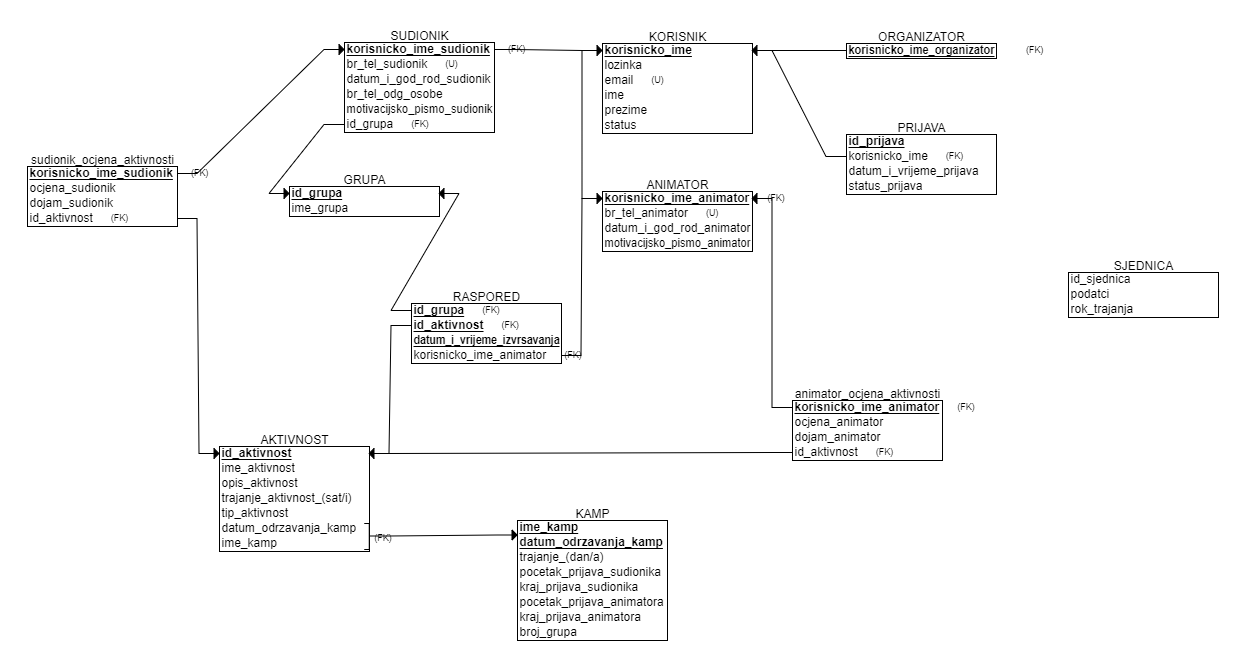
\includegraphics[width=\linewidth]{slike/ER_model_baze.png}}
				\caption{E-R dijagram baze podataka}
				\label{fig:ERdijagram}
			\end{figure}
			
			\eject
			
			
		\section{Dijagram razreda}
			
			\begin{figure}[H]
				\centerline{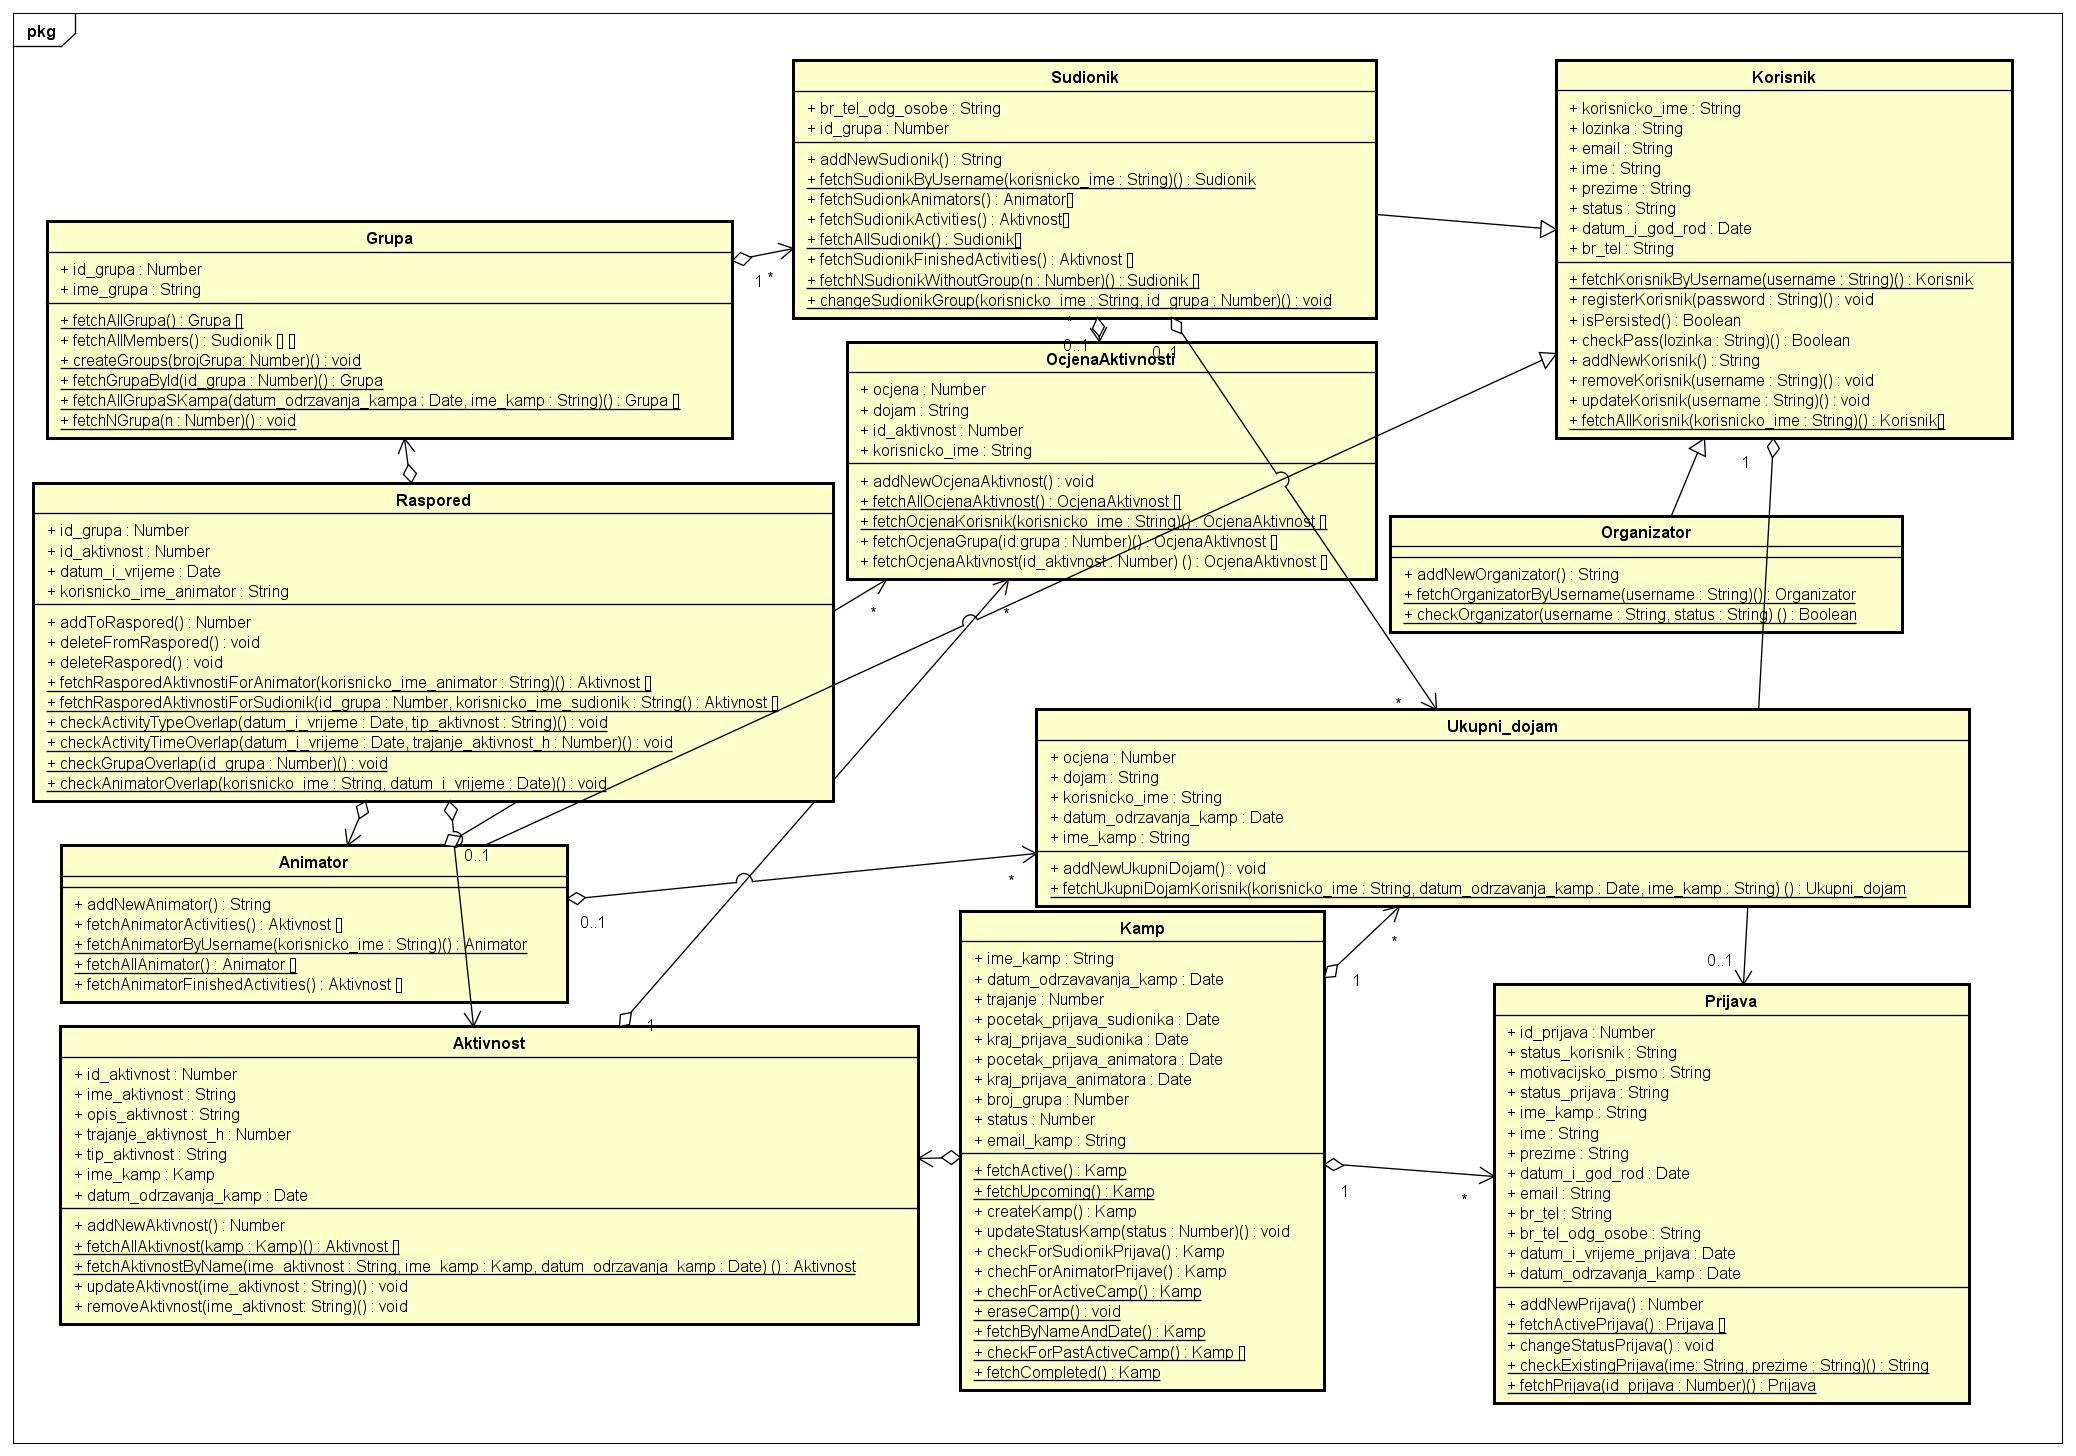
\includegraphics[width=\linewidth]{slike/Dijagram_razreda_modeli.png}}
				\caption{Dijagram razreda- modeli}
				\label{fig:dijagram_razreda_modeli}
			\end{figure}
			
			\eject
		
		\section{Dijagram stanja}
		
		Dijagram stanja prikazuje stanje objekta te prijelaze iz jednog stanja u drugo temeljene na događajima. Na slici 4.3 je prikazan dijagram stanja za registriranog sudionika. Nakon prijave, sudioniku se prikazuje početna stranica na kojoj se prikazuju sudionikov raspored te popis aktivnosti na kojima je sudjelovao. Sudionik može ocijeniti aktivnosti na kojima je sudjelovao, te po završetku kampa može ostaviti ukupni dojam. Također, sudionik može u izborniku odabrati neku od ponuđenih mogućnosti. Klikom na "Moj profil" prikazuju mu se njegovi osobni podatci. Klikom na "Moja grupa" prikazuju mu se podaci njegove grupe. Na slici 4.4 je prikazan dijagram stanja za organizatora. Nakon prijave, organizator na početnoj stranici može otvoriti izbornik te odabrati neku od ponuđenih mogućnosti. Klikom na "Stvori novi kamp" organizator može stvoriti novi kamp. Klikom na "Stvori novu aktivnost" organizator može stvoriti novu aktivnost. Klikom na "Prijave za kamp" organizator obrađuje pristigle prijave za kamp. Klikom na "Stvori Grupe" organizator može pregledati i stvoriti nove grupe te premjestiti sudionike. Klikom na "Moj profil" organizatoru se prikazuju njegovi osobni podatci.  
		\begin{figure}[H]
			\centerline{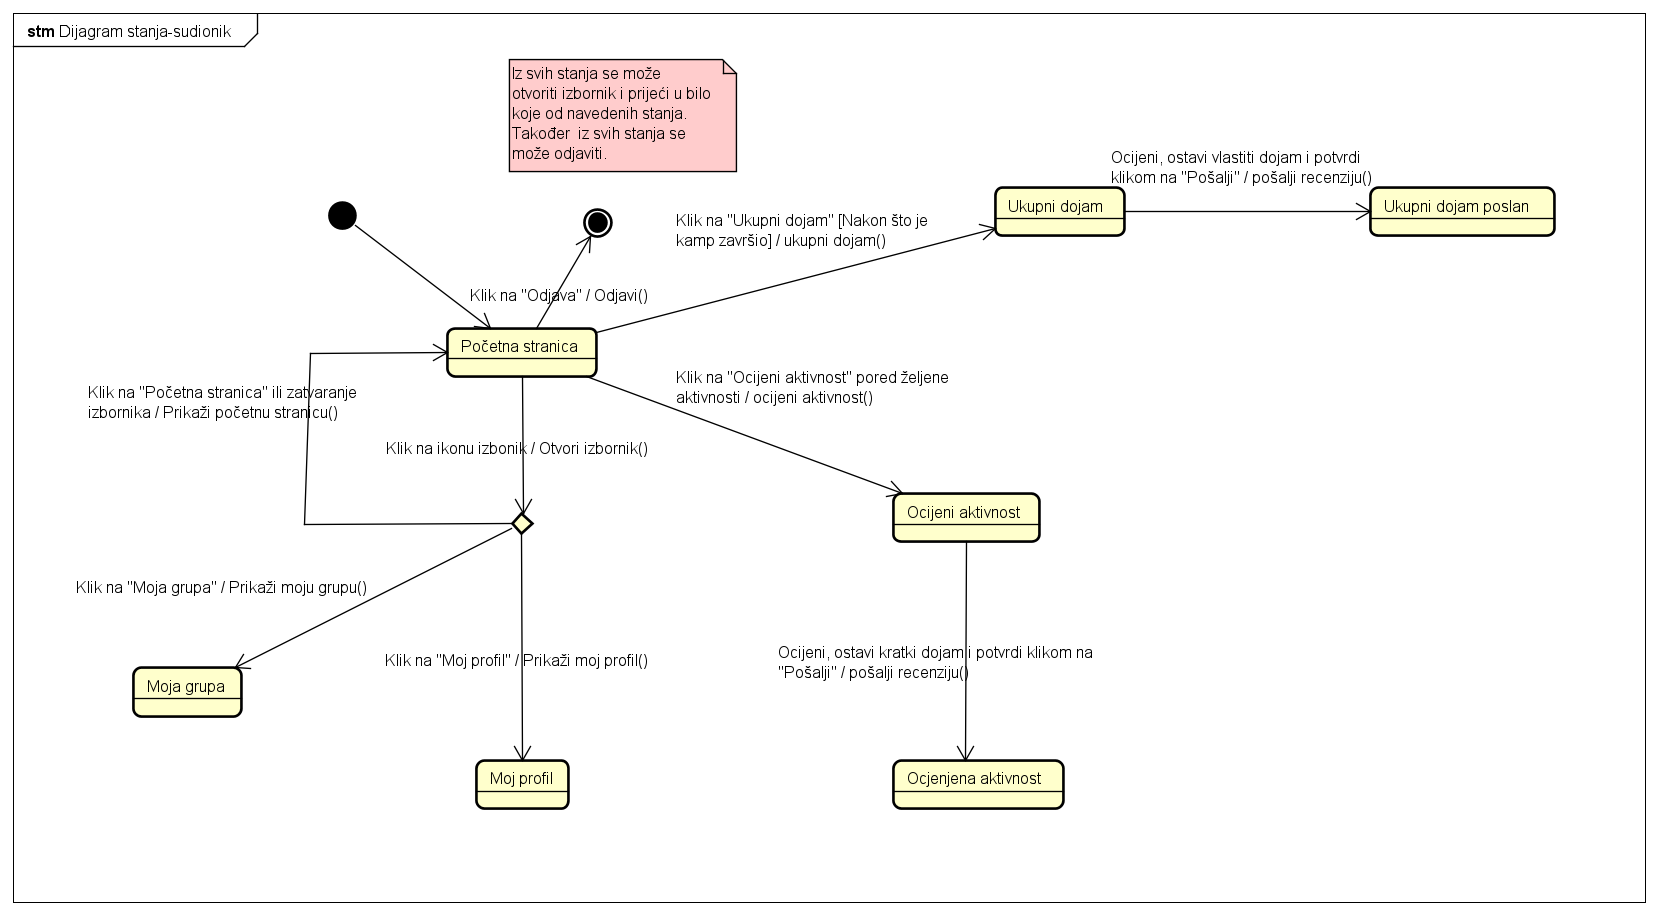
\includegraphics[width=\linewidth]{slike/Dijagram_stanja_sudionik.png}}
			\caption{Dijagram stanja- sudionik }
			\label{fig:dijagram_stanja_sudionik}
		\end{figure}
		
		\eject	
		
		\begin{figure}[H]
			\centerline{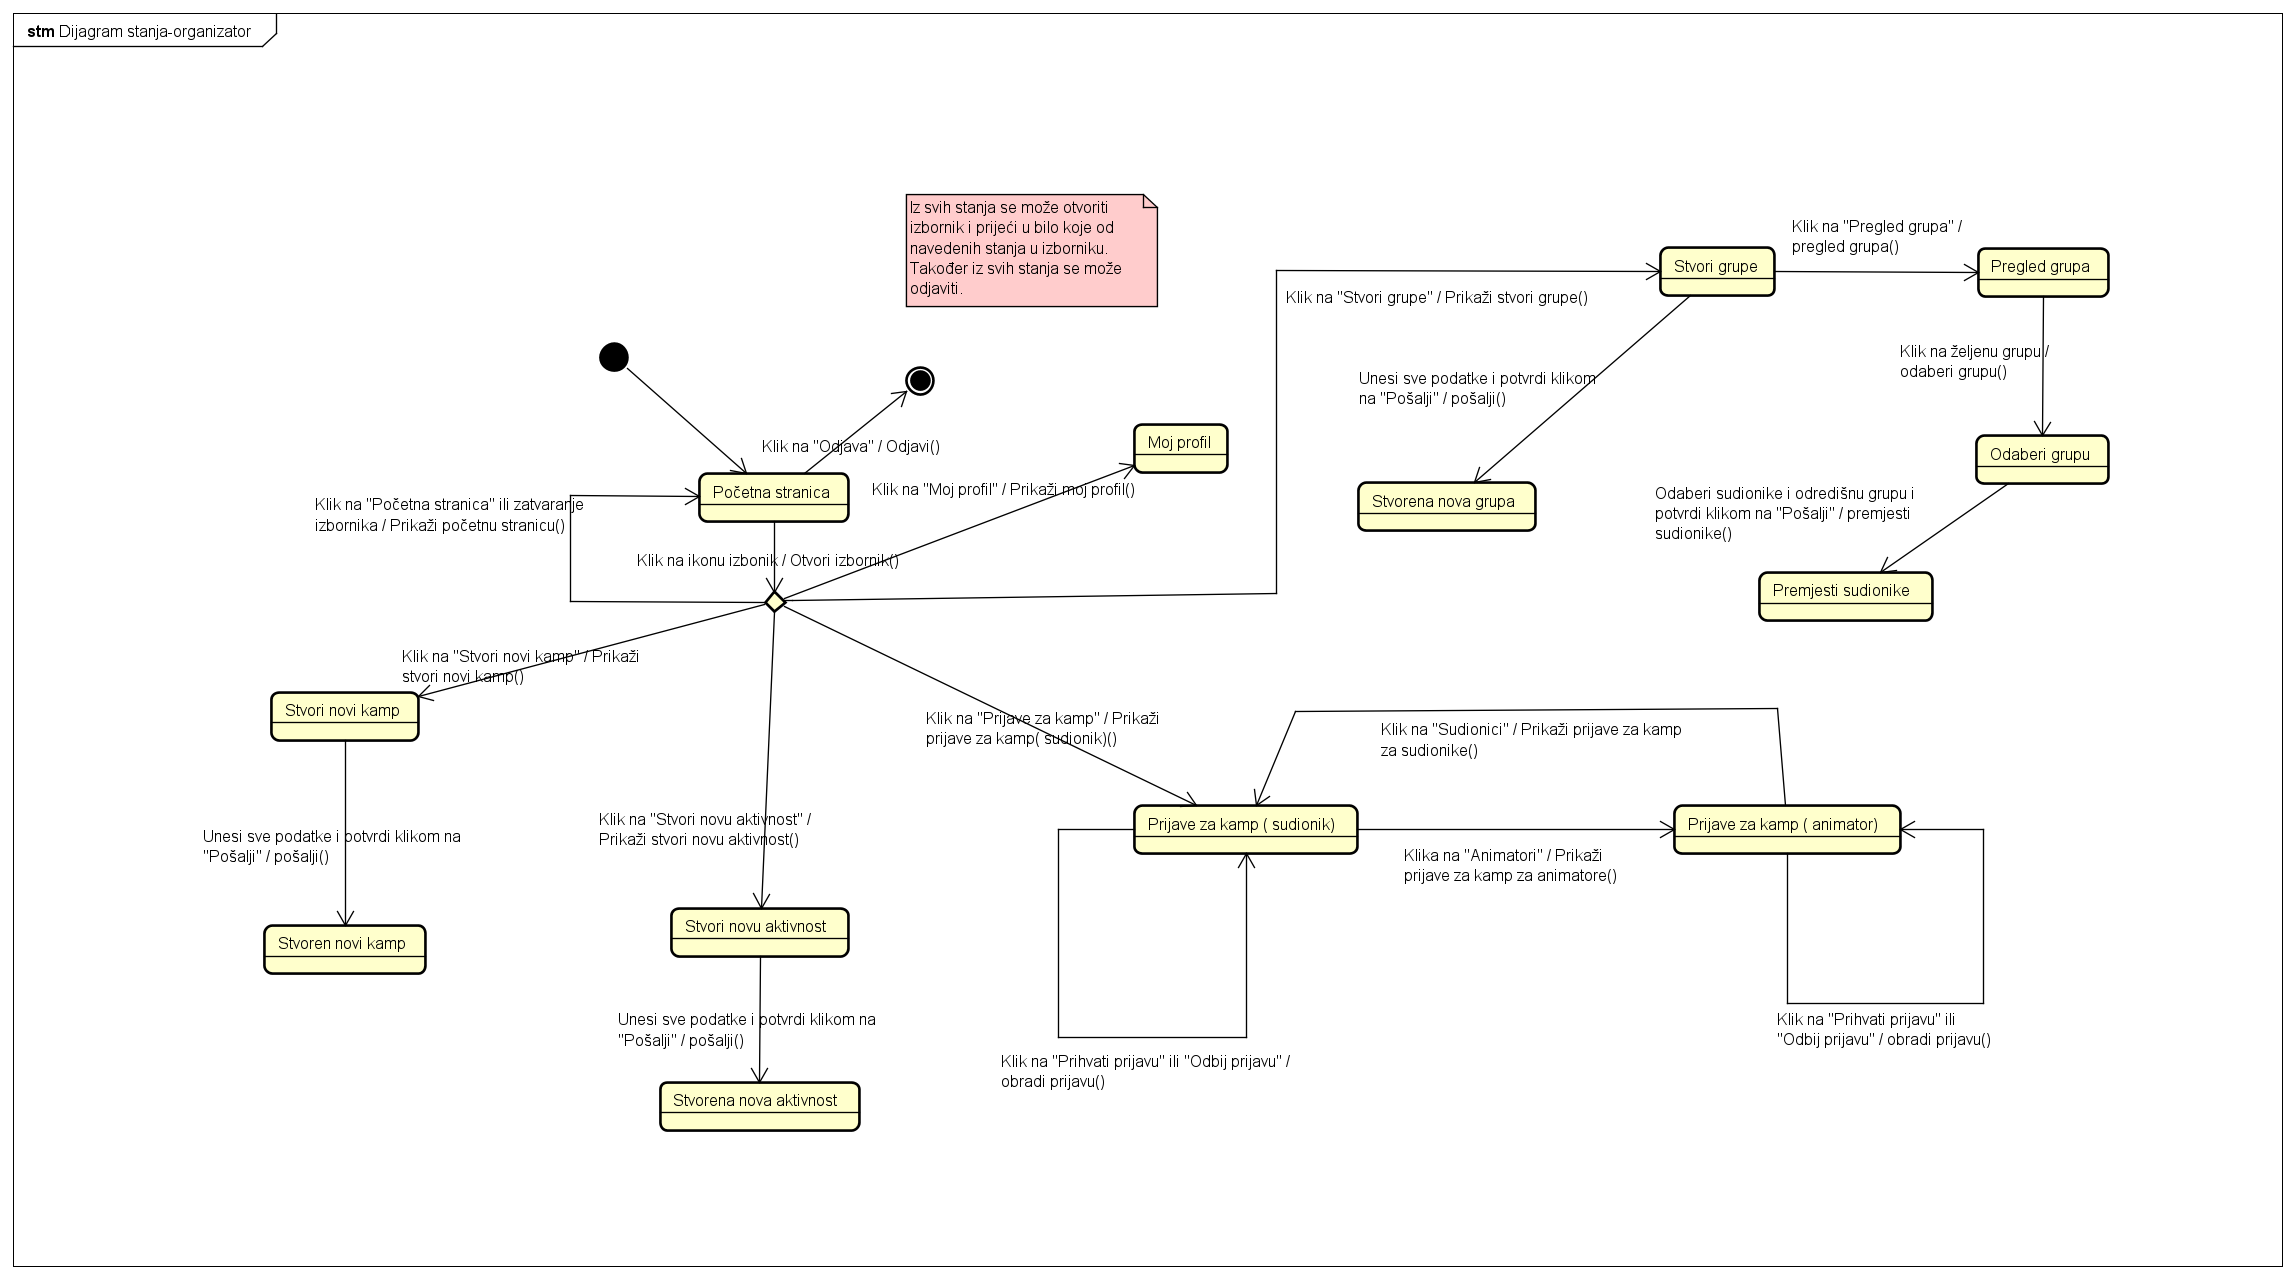
\includegraphics[width=\linewidth]{slike/Dijagram_stanja_organizator.png}}
			\caption{Dijagram stanja- organizator }
			\label{fig:dijagram_stanja_organizator}
		\end{figure}
		
		\eject			

		
	
	\chapter{Implementacija i korisničko sučelje}
		
		
		\section{Korištene tehnologije i alati}
		
			Komunikaciju u timu realizirana je korištenjem aplikacije WhatsApp(1). Za upravljanje podjele rada korištena je web platforma Asana(2). Za izradu UML dijagrama korišten je alat Astah Professional(3), a kao sustav za upravljanje izvornim kodom Git(4). Udaljeni repozitorij projekta dostupan je na web platformi GitLab(5). 
			Kao uređivač izvornog koda korišten je Visual Studio Code(6) tvrtke Microsoft. Neke od značajki ovog uređivača su debugiranje, naglašavanje sintakse, snippeti, refaktoriranje koda i ugrađeni git.
			Aplikacija je napisana koristeći radni okvir Express.js(7) i jezik JavaScript(8) za izradu backenda te React(9) i jezik JavaScript za izradu frontenda. React je biblioteka u JavaScriptu za izgradnju korisničkih sučelja, te se koristi u razvoju web i mobilnih aplikacija. Radni okvir Express se koristi za izgradnju web aplikacija i API-ja, pod licencom MIT-a.
			Kao sustav za upravljanje bazom podataka korišten je PostgreSQL(10) sustav. Njegove značajke su ACID svojstva. 
			
			Poveznice:
			\begin{packed_enum}	
				\item https://www.whatsapp.com/
				\item https://app.asana.com/
				\item https://astah.net/products/astah-professional/
				\item https://git-scm.com/
				\item https://about.gitlab.com/
				\item https://code.visualstudio.com/
				\item https://expressjs.com/
				\item https://www.javascript.com/
				\item https://reactjs.org/
				\item https://www.postgresql.org/
				
				
			\end{packed_enum}
			
			
			\eject 
		
	
		\section{Ispitivanje programskog rješenja}
			
			\textbf{\textit{dio 2. revizije}}\\
			
			 \textit{U ovom poglavlju je potrebno opisati provedbu ispitivanja implementiranih funkcionalnosti na razini komponenti i na razini cijelog sustava s prikazom odabranih ispitnih slučajeva. Studenti trebaju ispitati temeljnu funkcionalnost i rubne uvjete.}
	
			
			\subsection{Ispitivanje komponenti}
			\textit{Potrebno je provesti ispitivanje jedinica (engl. unit testing) nad razredima koji implementiraju temeljne funkcionalnosti. Razraditi \textbf{minimalno 6 ispitnih slučajeva} u kojima će se ispitati redovni slučajevi, rubni uvjeti te izazivanje pogreške (engl. exception throwing). Poželjno je stvoriti i ispitni slučaj koji koristi funkcionalnosti koje nisu implementirane. Potrebno je priložiti izvorni kôd svih ispitnih slučajeva te prikaz rezultata izvođenja ispita u razvojnom okruženju (prolaz/pad ispita). }
			
			
			
			\subsection{Ispitivanje sustava}
			
			 \textit{Potrebno je provesti i opisati ispitivanje sustava koristeći radni okvir Selenium\footnote{\url{https://www.seleniumhq.org/}}. Razraditi \textbf{minimalno 4 ispitna slučaja} u kojima će se ispitati redovni slučajevi, rubni uvjeti te poziv funkcionalnosti koja nije implementirana/izaziva pogrešku kako bi se vidjelo na koji način sustav reagira kada nešto nije u potpunosti ostvareno. Ispitni slučaj se treba sastojati od ulaza (npr. korisničko ime i lozinka), očekivanog izlaza ili rezultata, koraka ispitivanja i dobivenog izlaza ili rezultata.\\ }
			 
			 \textit{Izradu ispitnih slučajeva pomoću radnog okvira Selenium moguće je provesti pomoću jednog od sljedeća dva alata:}
			 \begin{itemize}
			 	\item \textit{dodatak za preglednik \textbf{Selenium IDE} - snimanje korisnikovih akcija radi automatskog ponavljanja ispita	}
			 	\item \textit{\textbf{Selenium WebDriver} - podrška za pisanje ispita u jezicima Java, C\#, PHP koristeći posebno programsko sučelje.}
			 \end{itemize}
		 	\textit{Detalji o korištenju alata Selenium bit će prikazani na posebnom predavanju tijekom semestra.}
			
			\eject 
		
		
		\section{Dijagram razmještaja}
			
			Dijagrami razmještaja opisuju topologiju sklopovlja i programsku potporu koja se koristi u implementaciji sustava u njegovom radnom okruženju. Na poslužiteljskom računalu se nalaze web poslužitelj i poslužitelj baze podataka. Klijenti koriste web preglednik za pristupanje web aplikaciji. Komunikacije između računala korisnika i poslužitelja odvija se putem HTTP veze.	
			\begin{figure}[H]
				\centerline{\includegraphics[width=\linewidth]{slike/dijagram_razmještaja.png}}
				\caption{Dijagram razmještaja}
				\label{fig:dijagram_razmjestaja}
			\end{figure}
			
			\eject 
		
		\section{Upute za puštanje u pogon}
		
			\textbf{\textit{dio 2. revizije}}\\
		
			 \textit{U ovom poglavlju potrebno je dati upute za puštanje u pogon (engl. deployment) ostvarene aplikacije. Na primjer, za web aplikacije, opisati postupak kojim se od izvornog kôda dolazi do potpuno postavljene baze podataka i poslužitelja koji odgovara na upite korisnika. Za mobilnu aplikaciju, postupak kojim se aplikacija izgradi, te postavi na neku od trgovina. Za stolnu (engl. desktop) aplikaciju, postupak kojim se aplikacija instalira na računalo. Ukoliko mobilne i stolne aplikacije komuniciraju s poslužiteljem i/ili bazom podataka, opisati i postupak njihovog postavljanja. Pri izradi uputa preporučuje se \textbf{naglasiti korake instalacije uporabom natuknica} te koristiti što je više moguće \textbf{slike ekrana} (engl. screenshots) kako bi upute bile jasne i jednostavne za slijediti.}
			
			
			 \textit{Dovršenu aplikaciju potrebno je pokrenuti na javno dostupnom poslužitelju. Studentima se preporuča korištenje neke od sljedećih besplatnih usluga: \href{https://aws.amazon.com/}{Amazon AWS}, \href{https://azure.microsoft.com/en-us/}{Microsoft Azure} ili \href{https://www.heroku.com/}{Heroku}. Mobilne aplikacije trebaju biti objavljene na F-Droid, Google Play ili Amazon App trgovini.}
			
			
			\eject 
	\chapter{Zaključak i budući rad}
		
		\textbf{\textit{dio 2. revizije}}\\
		
		 \textit{U ovom poglavlju potrebno je napisati osvrt na vrijeme izrade projektnog zadatka, koji su tehnički izazovi prepoznati, jesu li riješeni ili kako bi mogli biti riješeni, koja su znanja stečena pri izradi projekta, koja bi znanja bila posebno potrebna za brže i kvalitetnije ostvarenje projekta i koje bi bile perspektive za nastavak rada u projektnoj grupi.}
		
		 \textit{Potrebno je točno popisati funkcionalnosti koje nisu implementirane u ostvarenoj aplikaciji.}
		
		\eject 
	\chapter*{Popis literature}
		\addcontentsline{toc}{chapter}{Popis literature}
	 	
 		\textbf{\textit{Kontinuirano osvježavanje}}
	
		\textit{Popisati sve reference i literaturu koja je pomogla pri ostvarivanju projekta.}
		
		
		\begin{enumerate}
			
			
			\item  Programsko inženjerstvo, FER ZEMRIS, \url{http://www.fer.hr/predmet/proinz}
			
			\item  I. Sommerville, "Software engineering", 8th ed, Addison Wesley, 2007.
			
			\item  T.C.Lethbridge, R.Langaniere, "Object-Oriented Software Engineering", 2nd ed. McGraw-Hill, 2005.
			
			\item  I. Marsic, Software engineering book``, Department of Electrical and Computer Engineering, Rutgers University, \url{http://www.ece.rutgers.edu/~marsic/books/SE}
			
			\item  The Unified Modeling Language, \url{https://www.uml-diagrams.org/}
			
			\item  Astah Community, \url{http://astah.net/editions/uml-new}
		\end{enumerate}
		
		 
	
	
	\begingroup
	\renewcommand*\listfigurename{Indeks slika i dijagrama}
	%\renewcommand*\listtablename{Indeks tablica}
	%\let\clearpage\relax
	\listoffigures
	%\vspace{10mm}
	%\listoftables
	\endgroup
	\addcontentsline{toc}{chapter}{Indeks slika i dijagrama}


	
	\eject 
		
	\chapter*{Dodatak: Prikaz aktivnosti grupe}
		\addcontentsline{toc}{chapter}{Dodatak: Prikaz aktivnosti grupe}
		
		\section*{Dnevnik sastajanja}
		
		\textbf{\textit{Kontinuirano osvježavanje}}\\
		
		 \textit{U ovom dijelu potrebno je redovito osvježavati dnevnik sastajanja prema predlošku.}
		
		\begin{packed_enum}
			\item  sastanak
			
			\item[] \begin{packed_item}
				\item Datum: u ovom formatu: \today
				\item Prisustvovali: I.Prezime, I.Prezime
				\item Teme sastanka:
				\begin{packed_item}
					\item  opis prve teme
					\item  opis druge teme
				\end{packed_item}
			\end{packed_item}
			
			\item  sastanak
			\item[] \begin{packed_item}
				\item Datum: u ovom formatu: \today
				\item Prisustvovali: I.Prezime, I.Prezime
				\item Teme sastanka:
				\begin{packed_item}
					\item  opis prve teme
					\item  opis druge teme
				\end{packed_item}
			\end{packed_item}
			
			%
			
		\end{packed_enum}
		
		\eject
		\section*{Tablica aktivnosti}
		
			\textbf{\textit{Kontinuirano osvježavanje}}\\
			
			 \textit{Napomena: Doprinose u aktivnostima treba navesti u satima po članovima grupe po aktivnosti.}
					
						
			
			\begin{longtabu} to \textwidth {|X[7, l]|X[1, c]|X[1, c]|X[1, c]|X[1, c]|X[1, c]|X[1, c]|X[1, c]|}
								
				\cline{2-8} \multicolumn{1}{c|}{\textbf{}} &     \multicolumn{1}{c|}{\rotatebox{90}{\textbf{Ime Prezime voditelja }}} & \multicolumn{1}{c|}{\rotatebox{90}{\textbf{Ime Prezime }}} &	\multicolumn{1}{c|}{\rotatebox{90}{\textbf{Ime Prezime }}} &	\multicolumn{1}{c|}{\rotatebox{90}{\textbf{Ime Prezime }}} &
				\multicolumn{1}{c|}{\rotatebox{90}{\textbf{Ime Prezime }}} &
				\multicolumn{1}{c|}{\rotatebox{90}{\textbf{Ime Prezime }}} &	\multicolumn{1}{c|}{\rotatebox{90}{\textbf{Ime Prezime }}} \\ \hline 
				\endfirsthead
				
			
				\cline{2-8} \multicolumn{1}{c|}{\textbf{}} &     \multicolumn{1}{c|}{\rotatebox{90}{\textbf{Ime Prezime voditelja}}} & \multicolumn{1}{c|}{\rotatebox{90}{\textbf{Ime Prezime }}} &	\multicolumn{1}{c|}{\rotatebox{90}{\textbf{Ime Prezime }}} &
				\multicolumn{1}{c|}{\rotatebox{90}{\textbf{Ime Prezime }}} &	\multicolumn{1}{c|}{\rotatebox{90}{\textbf{Ime Prezime }}} &
				\multicolumn{1}{c|}{\rotatebox{90}{\textbf{Ime Prezime }}} &	\multicolumn{1}{c|}{\rotatebox{90}{\textbf{Ime Prezime }}} \\ \hline 
				\endhead
				
				
				\endfoot
							
				 
				\endlastfoot
				
				Upravljanje projektom 		&  &  &  &  &  &  & \\ \hline
				Opis projektnog zadatka 	&  &  &  &  &  &  & \\ \hline
				
				Funkcionalni zahtjevi       &  &  &  &  &  &  &  \\ \hline
				Opis pojedinih obrazaca 	&  &  &  &  &  &  &  \\ \hline
				Dijagram obrazaca 			&  &  &  &  &  &  &  \\ \hline
				Sekvencijski dijagrami 		&  &  &  &  &  &  &  \\ \hline
				Opis ostalih zahtjeva 		&  &  &  &  &  &  &  \\ \hline

				Arhitektura i dizajn sustava	 &  &  &  &  &  &  &  \\ \hline
				Baza podataka				&  &  &  &  &  &  &   \\ \hline
				Dijagram razreda 			&  &  &  &  &  &  &   \\ \hline
				Dijagram stanja				&  &  &  &  &  &  &  \\ \hline
				Dijagram aktivnosti 		&  &  &  &  &  &  &  \\ \hline
				Dijagram komponenti			&  &  &  &  &  &  &  \\ \hline
				Korištene tehnologije i alati 		&  &  &  &  &  &  &  \\ \hline
				Ispitivanje programskog rješenja 	&  &  &  &  &  &  &  \\ \hline
				Dijagram razmještaja			&  &  &  &  &  &  &  \\ \hline
				Upute za puštanje u pogon 		&  &  &  &  &  &  &  \\ \hline 
				Dnevnik sastajanja 			&  &  &  &  &  &  &  \\ \hline
				Zaključak i budući rad 		&  &  &  &  &  &  &  \\  \hline
				Popis literature 			&  &  &  &  &  &  &  \\  \hline
				&  &  &  &  &  &  &  \\ \hline \hline
				\textit{Dodatne stavke kako ste podijelili izradu aplikacije} 			&  &  &  &  &  &  &  \\ \hline
				\textit{npr. izrada početne stranice} 				&  &  &  &  &  &  &  \\ \hline 
				\textit{izrada baze podataka} 		 			&  &  &  &  &  &  & \\ \hline 
				\textit{spajanje s bazom podataka} 							&  &  &  &  &  &  &  \\ \hline
				\textit{back end} 							&  &  &  &  &  &  &  \\  \hline
				 							&  &  &  &  &  &  &\\  \hline
				
				
			\end{longtabu}
					
					
		\eject
		\section*{Dijagrami pregleda promjena}
		
		\textbf{\textit{dio 2. revizije}}\\
		
		\textit{Prenijeti dijagram pregleda promjena nad datotekama projekta. Potrebno je na kraju projekta generirane grafove s gitlaba prenijeti u ovo poglavlje dokumentacije. Dijagrami za vlastiti projekt se mogu preuzeti s gitlab.com stranice, u izborniku Repository, pritiskom na stavku Contributors.}
		
	


\end{document} %naredbe i tekst nakon ove naredbe ne ulaze u izgrađen dokument 


